%----------------------------------------------------------------------------------------
%	DOCUMENT CONFIGURATIONS
%----------------------------------------------------------------------------------------
\documentclass[11pt]{article}

\usepackage{float}
\usepackage{caption}
\usepackage{subcaption}
\usepackage{cleveref}

\RequirePackage{amsmath}
\RequirePackage{amssymb}
\RequirePackage{amsthm}
\usepackage{amsfonts}
\usepackage{mathtools}

\usepackage{epsfig}
\usepackage{amscd}
\usepackage{graphicx}% Include figure files
\usepackage{dcolumn}% Align table columns on decimal point
\usepackage{bm}% bold math
\usepackage{enumerate}
\usepackage{tikz}


\usepackage[top=1.5in,bottom=1.5in,right=1.5in, left=1.5in]{geometry}

\captionsetup[subfigure]{subrefformat=simple,labelformat=simple}
\renewcommand\thesubfigure{(\alph{subfigure})}

%----------------------------------------------------------------------------------------
%	TITLE SECTION
%----------------------------------------------------------------------------------------



%----------------------------------------------------------------------------------------
%	ARTICLE SECTION
%----------------------------------------------------------------------------------------

\begin{document}

\author{Meilei Jiang\\
    Department of Statistics and Operations Research\\
		University of North Carolina at Chapel Hill}
\title{Simulation study: Modified SVA versus IRW-SVA}

\maketitle
\section{Modified SVA}
Papers \cite{leek2012sva, leek2007capturing, leek2008general} proposed a factor model for the relationship between expression values $X$, measured biological factors $S$, and unmeasured biological and non-biological factors $G$:
$$ \begin{aligned}
X = B S + \Gamma G + U.
\end{aligned}$$
In the model, $X_{m \times n}$ is a data matrix where each entry $x_{ij}$ is the value of gene $i$ for sample $j$, $S_{p_1 \times n}$ is a design model matrix of $p_1$ measured factors for the $n$ samples, $B_{m \times p_1}$ are the coefficients for these variables on the $m$ genes, $G_{p_2 \times n}$ is an unknown matrix that parameterizes the effect of unmeasured confounders and $\Gamma_{m \times p_2}$ is the corresponding coefficient matrix for $G$.

In order to remove the batch effects, iteratively reweighted surrogate variable analysis (IRW-SVA) is proposed to estimate $G$. An essential idea of SVA is to identify a subset of genes that are strongly associated with unmeasured confounders, but not with the group outcome. Especially, an empirical Bayesian procedure has been applied to estimate the posterior probabilities of each gene affected by unmeasured confounders and measured factors, namely: 
$$\begin{aligned}
\pi_{i\gamma} &= \text{Pr}( \gamma_i \neq \vec{0}| X, S, \hat{G}) \\
\pi_{i b} &= \text{Pr}(b_i \neq \vec{0} | \gamma_i \neq \vec{0}, X, S, \hat{G}) 
\end{aligned}$$
Next the probability that a gene is associated with unmeasured confounders but not with the measured factors is calculated
$$\begin{aligned}
\pi_{i w} &= \text{Pr}(b_i = \vec{0} \text{ } \& \text{ } \gamma_i \neq \vec{0} | X, S, \hat{G}) \\
&= \text{Pr}(b_i = \vec{0} | \gamma_i \neq \vec{0}, X, S, \hat{G}) \text{Pr}( \gamma_i \neq \vec{0}| X, S, \hat{G}) \\
&= (1 - \pi_{i b})\pi_{i\gamma}                     
\end{aligned}$$
In IRW-SVA, $\pi_{i w}$ is used to weight the $i$th row of $X$ and a singular value decomposition on the weighted $X$ is performed to reconstruct $\hat{G}$.

However, if we estimate $\hat{G}$ using this approach, I think it assumes there exists such a subset of genes in the data set. When such a subset does not exist, IRW-SVA can fail, as shown in Case 1 of the simulation study.

There seems to be a simple way to overcome this problem: use the probability $\pi_{i \gamma}$ to weight the $i$th row of the residual matrix $R = X - \hat{B} S$. Then reconstruct $\hat{G}$ through the singular value decomposition of the weighted $R$. 


In order to investigate this idea, a simple simulation study is set up to compare the performance of these two approaches to SVA.

\section{Simulation Settings} 

Data matrix has the dimensions of 100 $\times$ 80, i.e. 100 genes and 80 samples, as shown in Figure~\ref{fig:heatmap}. The 80 Samples (columns) come from two classes (the measured factor) and two batches (the unmeasured factor)
\begin{itemize} 
\item Class 1: Samples 1 - 40; Class 2: Samples 41 - 80.
\item Batch 1: Samples 1 - 20, 41 - 60; Batch 2: Samples 21 - 40, 61 - 80.
\end{itemize}
This results in the design model matrix $S = \begin{pmatrix}
1_{40} & 1_{40} \\
1_{40} & 0_{40} 
\end{pmatrix}$ and the confounder matrix $G = \begin{pmatrix}
1_{20} & 0_{20} & 1_{20} & 0_{20} 
\end{pmatrix}$, where $1_{k}$ $(0_{k})$ is the $1 \times k$ row vector of all ones (zeros respectively).

The 100 Genes (rows) have four types, which are shown in separate panels of Figure~\ref{fig:heatmap}:
\begin{itemize}
\item Type A: Genes with class label (measured factor) but not with batch label (unmeasured factor) signal.
\item Type B: Genes with batch label (unmeasured factor) but not with class label (measured factor) signal.
\item Type C: Genes with both class label (measured factor) and batch label (unmeasured factor) signal.
\item Type D: Genes with no signal.
\end{itemize}


The key step of IRW-SVA is to identify the Type B genes and use them as the focus of estimating $G$. In the simulation study, two cases are typically investigated:
\begin{itemize}
\item Case 1: Simulation data set does not contain Type B genes.
\item Case 2: Simulation data set contains Type B genes.
\end{itemize}

\begin{figure}[h!]
    \centering
    \begin{subfigure}[t]{0.4\textwidth}
    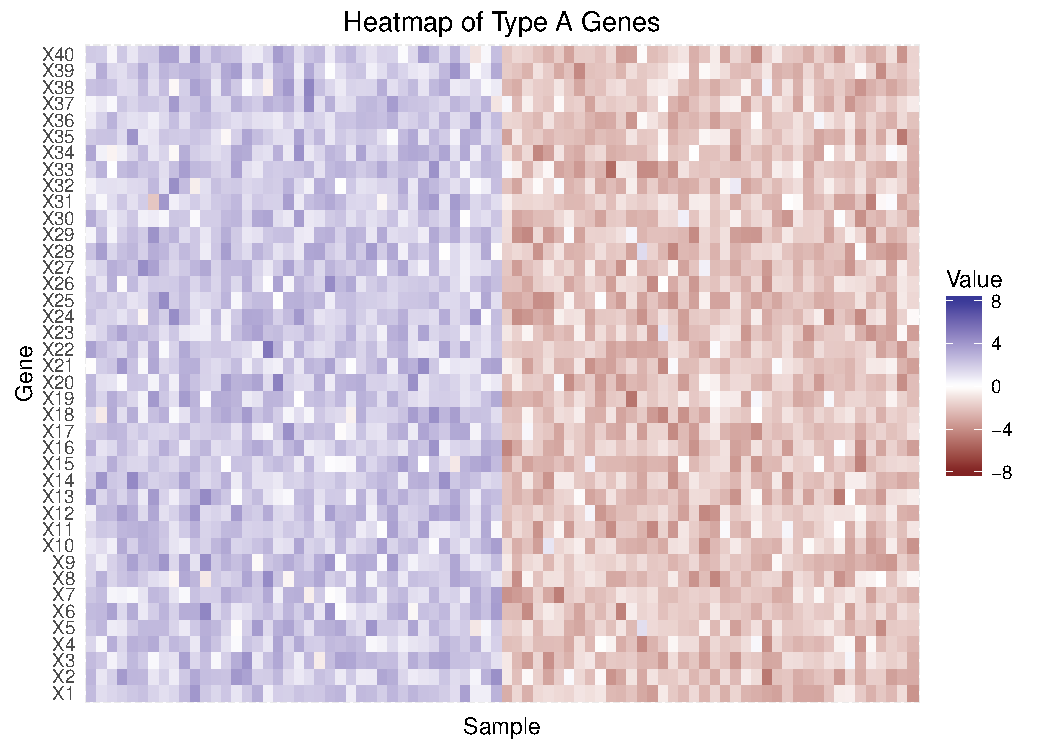
\includegraphics[width = \textwidth]{figures/Type_A_Gene.pdf}
    \caption{Type A: class, no batch signal.}
    \label{fig:type_a}
    \end{subfigure}
    ~
    \centering
    \begin{subfigure}[t]{0.4\textwidth}
    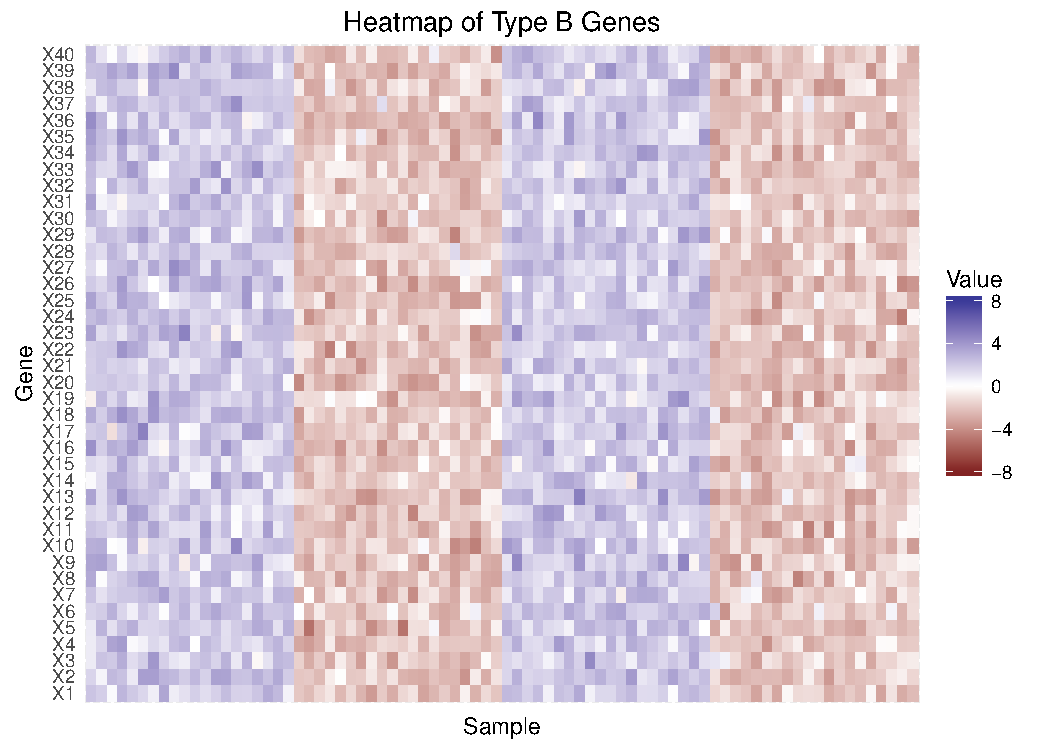
\includegraphics[width = \textwidth]{figures/Type_B_Gene.pdf}
    \caption{Type B: batch no class signal.}
    \label{fig:type_b}
    \end{subfigure}
    \\
    \centering
    \begin{subfigure}[t]{0.4\textwidth}
    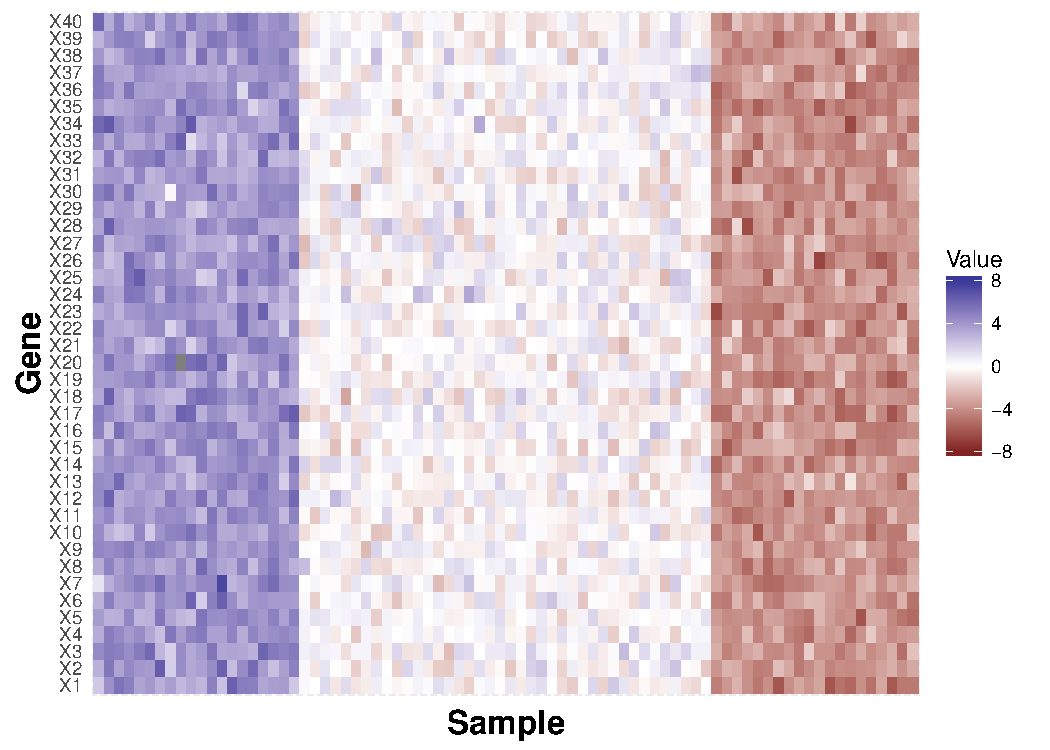
\includegraphics[width = \textwidth]{figures/Type_C_Gene.pdf}
    \caption{Type C: both class and batch signal.}
     \label{fig:type_c}
   \end{subfigure}
    ~
    \centering
    \begin{subfigure}[t]{0.4\textwidth}
    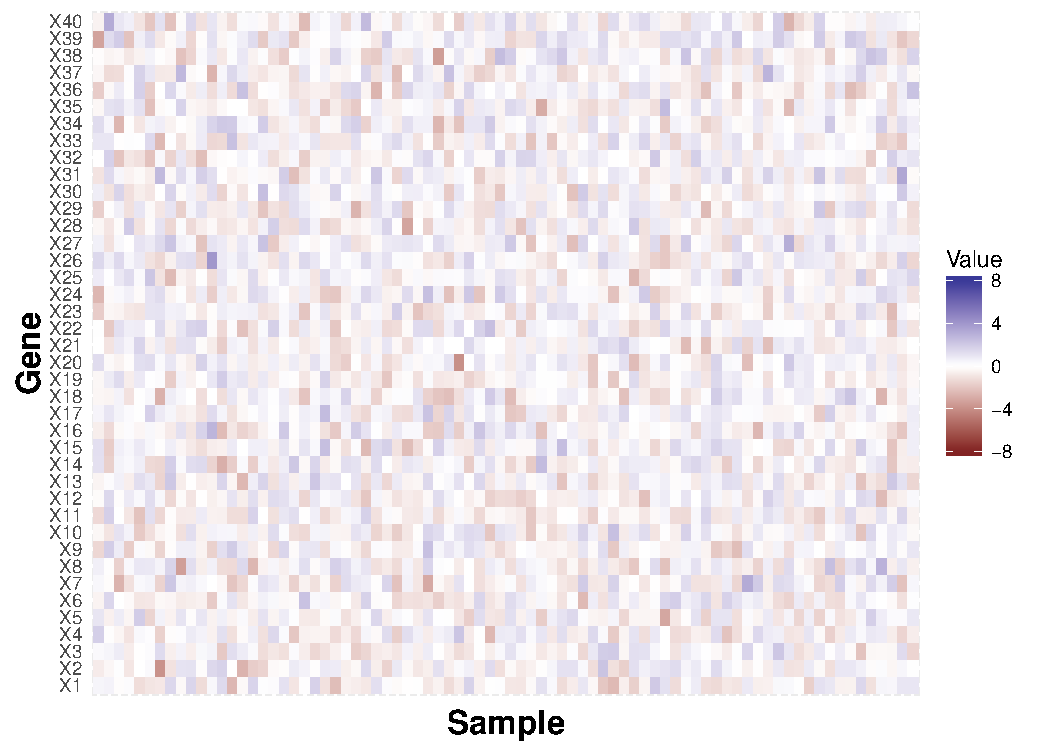
\includegraphics[width = \textwidth]{figures/Type_D_Gene.pdf}
    \caption{Type D: no signal.}
    \label{fig:type_d}
    \end{subfigure}
    \caption{Separate heatmaps for each of the four gene types determining on class and batch labels. The rows are genes, the columns are samples, and the entries are color coded expression values.}
    \label{fig:heatmap}
\end{figure}



\newpage
\section{Simulation Result}

\subsection{Case 1: Type C and Type D Genes.}

The input data matrix in Case 1 is shown in Figure~\ref{fig:svas1}\subref{fig:data1}, which is the concatenation of the matrices in Figure~\ref{fig:heatmap}\subref{fig:type_c} and Figure~\ref{fig:heatmap}\subref{fig:type_d}. Figure~\ref{fig:svas1}\subref{fig:sva1} shows that the data matrix after batch adjusting using IRW-SVA still retains the same pattern as the original simulation data set, which indicates that IRW-SVA failed to adjust for batch effects in this case. Figure~\ref{fig:svas1}\subref{fig:new_sva1} shows that after batch adjustment using modified SVA, the rows of Type C genes in the data set, which are affected by both class and batch effects, have been recovered as the class signal in Figure~\ref{fig:heatmap}\subref{fig:type_a}. This indicates that modified SVA adjusts batch effects and recovers the pattern of the measured factors quite well in Case 1. 

In order to understand the failure of IRW-SVA in Case 1, the posterior probabilities are investigated in the two approaches to SVA. In Figure~\ref{fig:visual1}, the x-axes and y-axes represent the gene index and the estimated probabilities respectively, and the genes are colored by their types. Figures~\ref{fig:visual1}\subref{fig:pprob1_1} and~\ref{fig:visual1}\subref{fig:pprob1_2} show the posterior probabilities, i.e. $\pi_{i b}$ and $\pi_{i \gamma}$, of each gene affected by class effects and batch effects respectively. In both subfigures we expect that Type C genes have high probabilities while Type D genes have low probabilities. In Figure~\ref{fig:visual1}\subref{fig:pprob1_1} the Type C genes are all nearly 1 and the Type D genes are usually near 0, which indicates that both IRW-SVA and modified SVA correctly identify the genes affected by class effects. In the left panel of Figure~\ref{fig:visual1}\subref{fig:pprob1_2} almost all the genes are near zero and only several Type D genes are nearly 1. This shows that IRW-SVA does not correctly identify the genes associated with batch label, while the right panel of Figure~\ref{fig:visual1}\subref{fig:pprob1_2} indicates modified SVA is able to do that. This is not surprising since IRW-SVA relies on Type B Genes to recover batch label signal but the data set in Case 1 does not contain Type B genes.

Moreover, Figure~\ref{fig:vector1} visualizes the values of the surrogate variables constructed by the two approaches to SVA respectively for each sample. In Figure~\ref{fig:vector1}, x-axes and y-axes represent samples and expression value respectively, and samples are colored by batch labels. The right panel of Figure~\ref{fig:vector1} shows that the samples from two batches are quite separable using the surrogate variable calculated by the modified SVA, but the left panel of Figure~\ref{fig:vector1} shows no useful separation by IRW-SVA. 

All these results in Case 1 indicate that modified SVA has better performance than IRW-SVA when Type B genes do not exist in the data.

\begin{figure}[h!]
    \centering
    \begin{subfigure}[b]{0.31\textwidth}
        \centering
        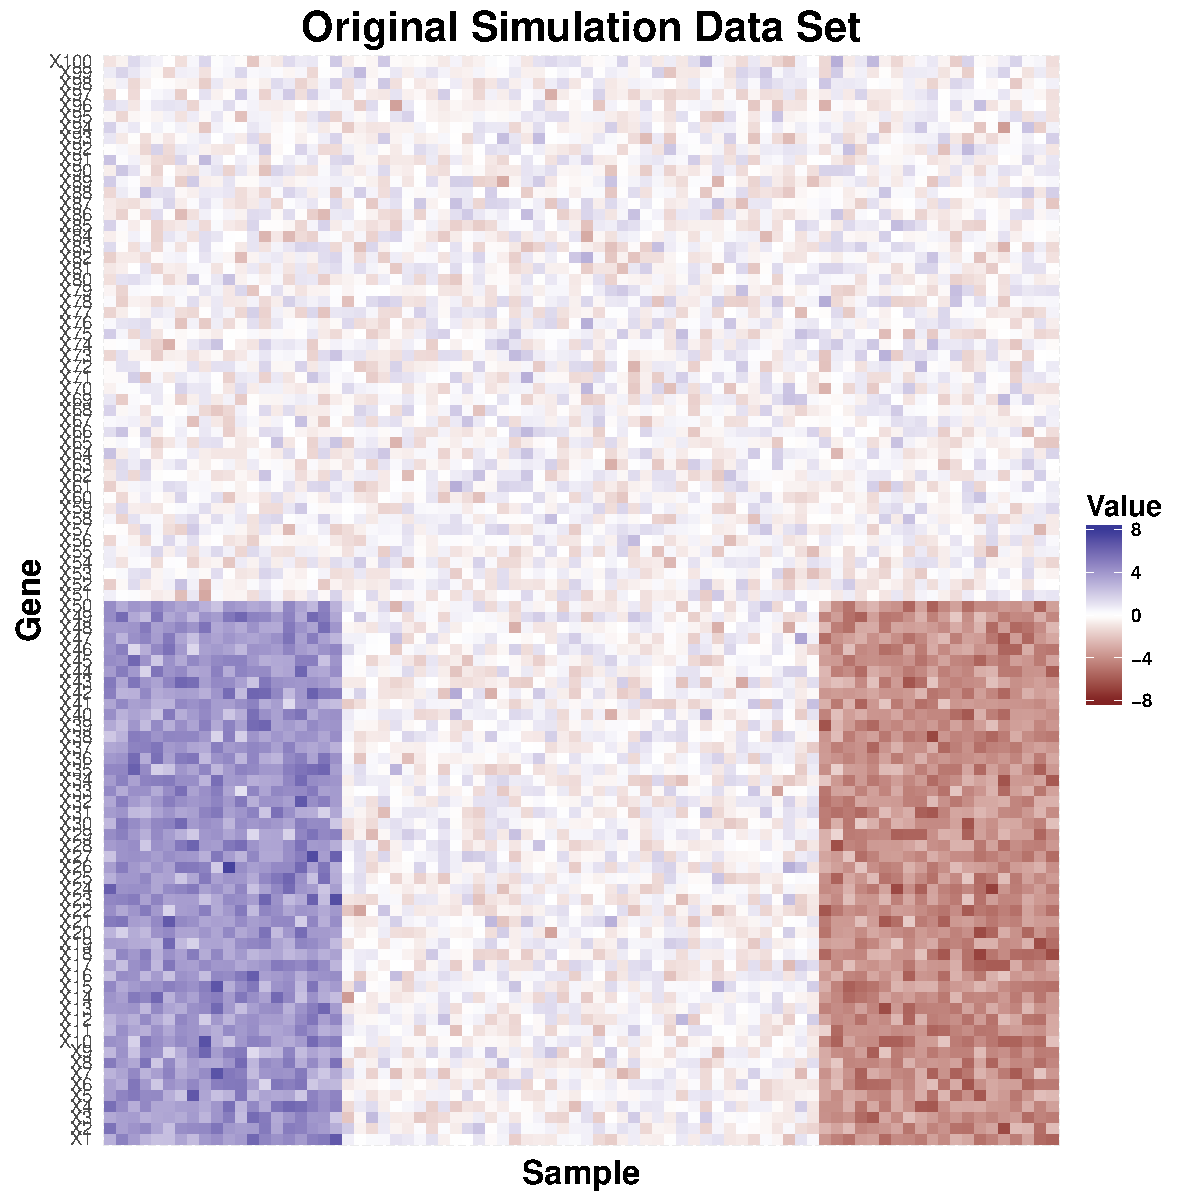
\includegraphics[width = \textwidth]{figures/simulate1.pdf}
        \caption{Original simulation data set in the Case 1}
        \label{fig:data1}
    \end{subfigure}% 
~
    \begin{subfigure}[b]{0.31\textwidth}
        \centering
        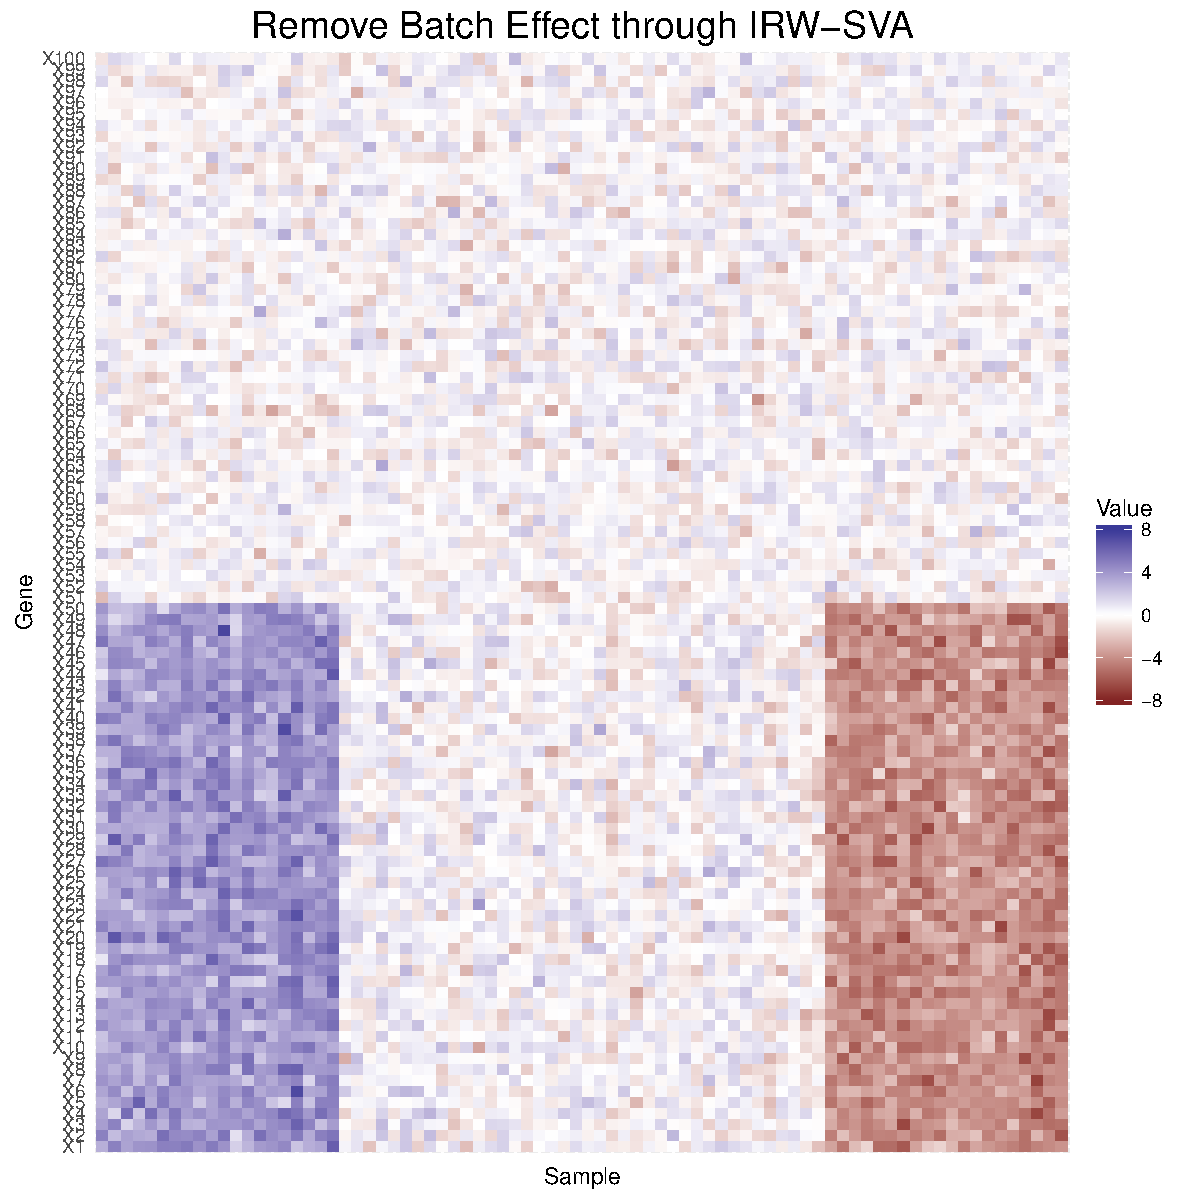
\includegraphics[width = \textwidth]{figures/sva1.pdf}
        \caption{Batch adjustment by IRW-SVA}
        \label{fig:sva1}
    \end{subfigure}  %
~
    \begin{subfigure}[b]{0.31\textwidth}
        \centering
        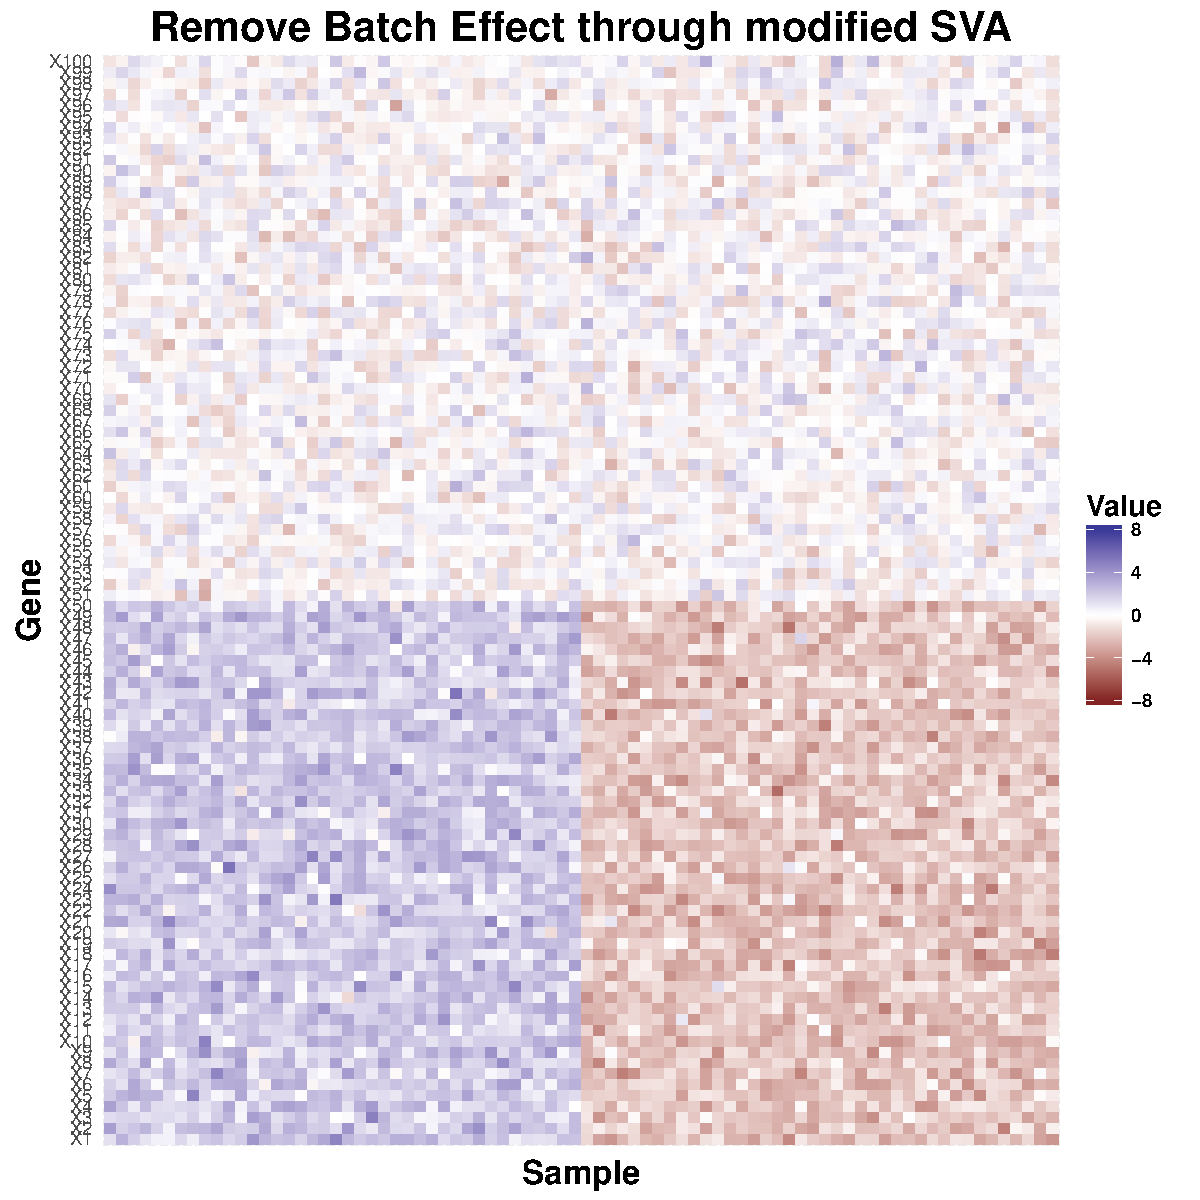
\includegraphics[width = \textwidth]{figures/new_sva1.pdf}
        \caption{Batch adjustment by modified SVA}
        \label{fig:new_sva1}
    \end{subfigure}    
    \caption{Study batch effect through two approaches to SVA in Case 1. Show failure of IRW-SVA in this case.}
    \label{fig:svas1}
\end{figure}




\begin{figure}[h!]
    \centering
    \begin{subfigure}[t]{0.45\textwidth}
    \centering
    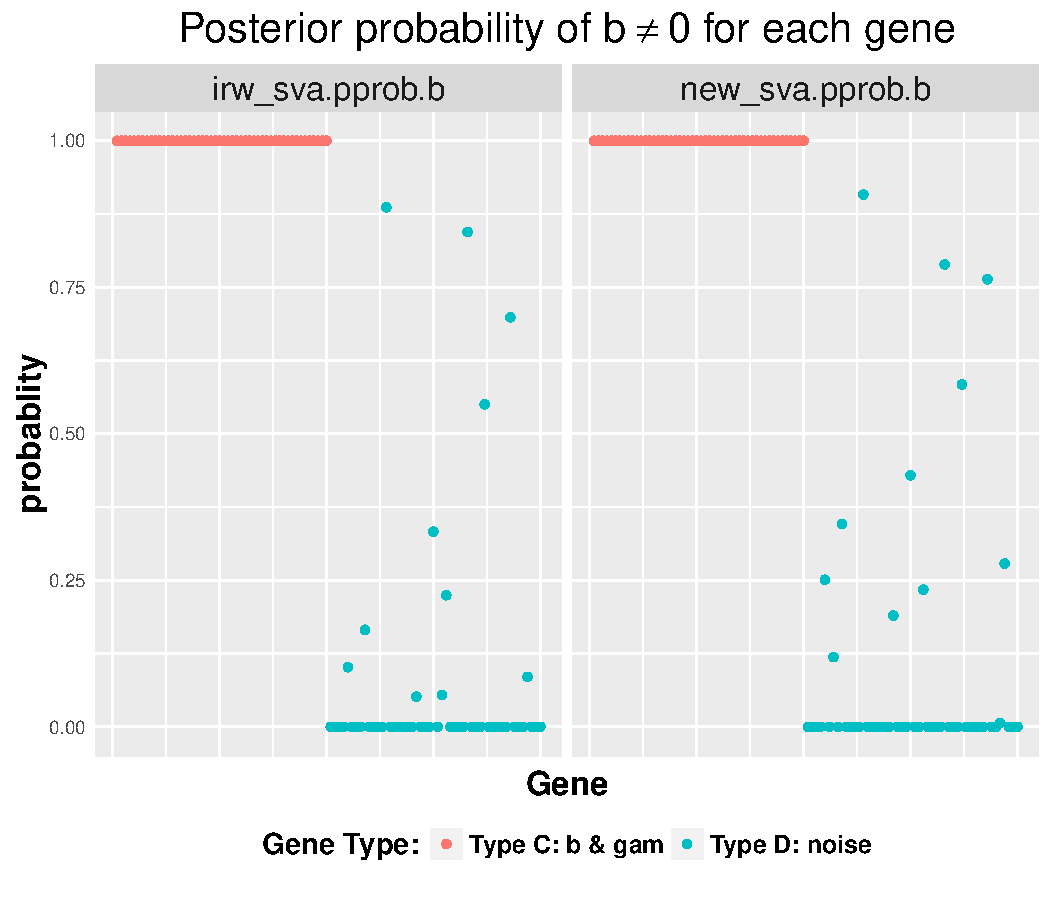
\includegraphics[width = \textwidth]{figures/pprop1_2.pdf}
    \caption{Posterior probability of genes affected by class label (measured factor).}
    \label{fig:pprob1_1}
    \end{subfigure}
    ~
     \begin{subfigure}[t]{0.45\textwidth}
    \centering
    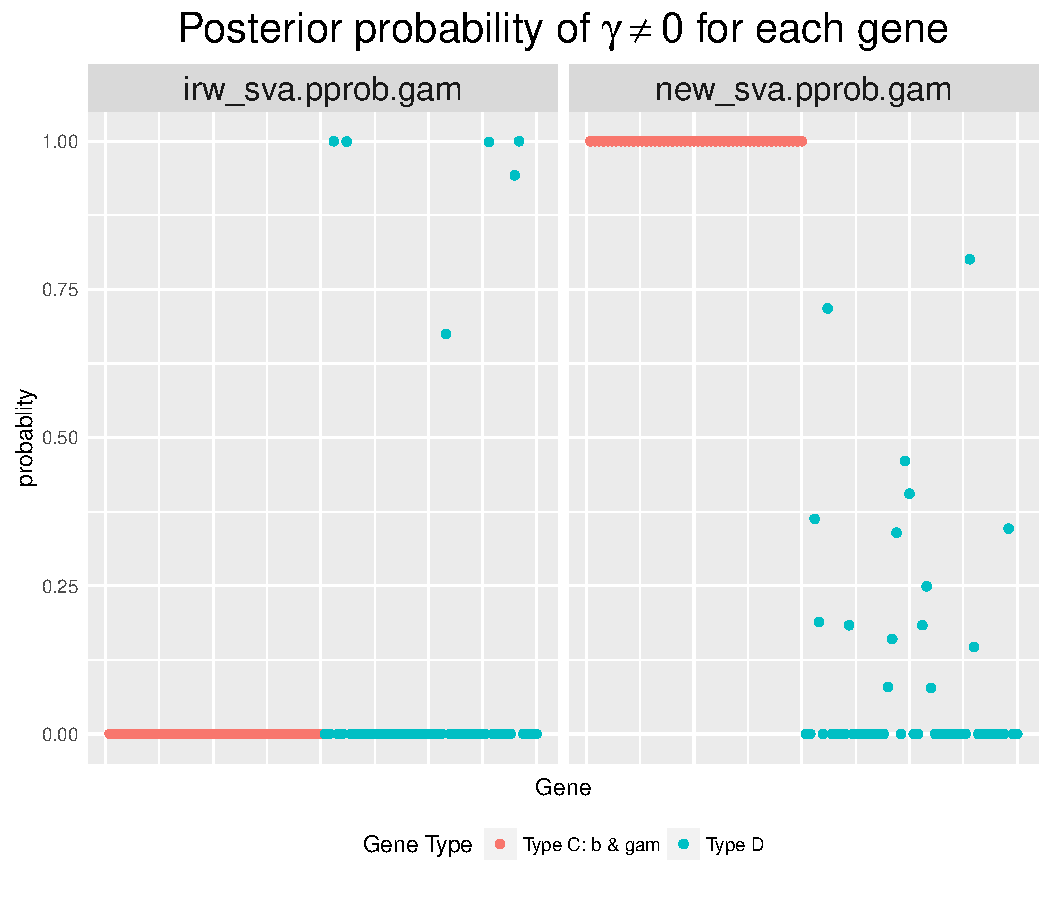
\includegraphics[width = \textwidth]{figures/pprop1_1.pdf}
    \caption{Posterior probability of genes affected by batch label (unmeasured factor).}
    \label{fig:pprob1_2}
    \end{subfigure}
    \caption{The posterior probabilities for genes in Case 1. In each subfigure, the panels on the left show the results from IRW-SVA and the panels on the right show the results from modified SVA.}
    \label{fig:visual1}
\end{figure}

\begin{figure}
    \centering
    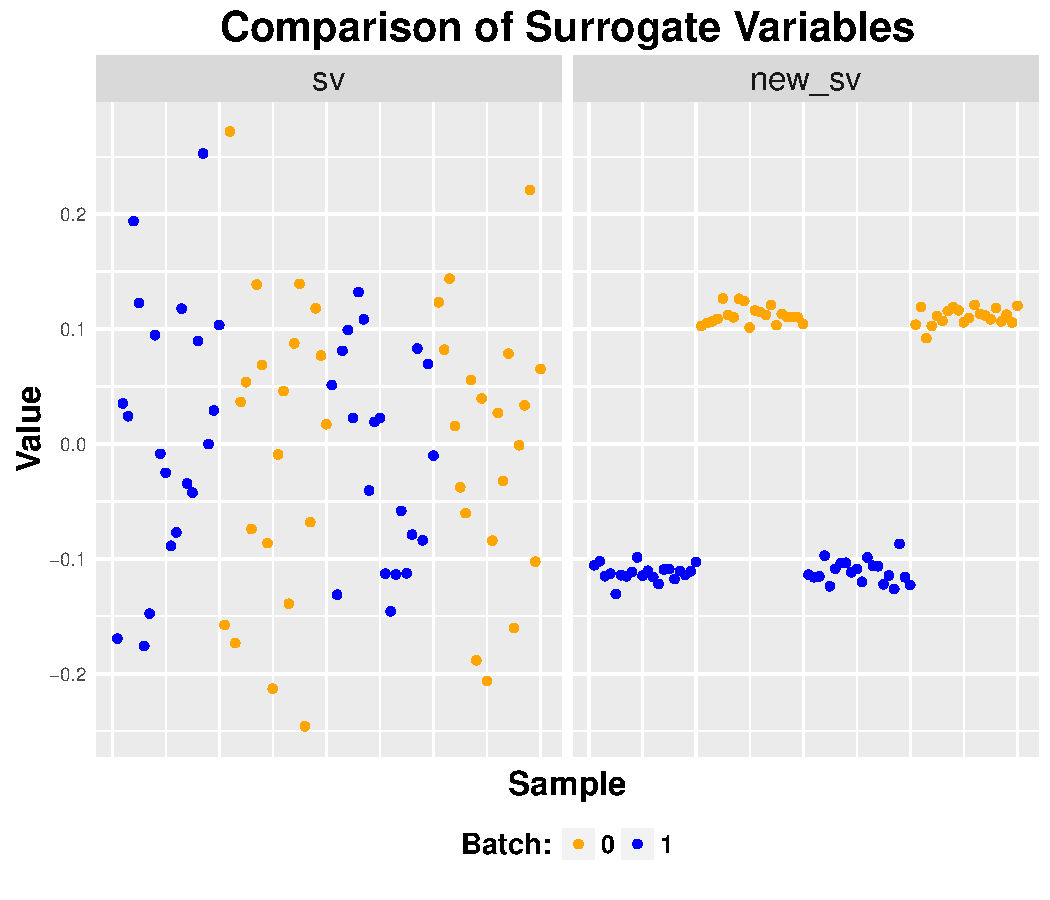
\includegraphics[width = 0.6\textwidth]{figures/vector1.pdf}
    \caption{Comparison of surrogate variables. The left panel shows the surrogate variable constructed through IRW-SVA and the right panel shows the surrogate variable constructed through modified SVA. Modified SVA gives much better performance.}
    \label{fig:vector1}
\end{figure}

\newpage

\subsection{Case 2: All four types of genes.}

In contrast to Case 1, the input data matrix in Case 2 contains all four types of genes, as shown in Figure~\ref{fig:svas2}\subref{fig:data2}, which is a typical situation we expect IRW-SVA works. Figure~\ref{fig:svas2}\subref{fig:sva2} and Figure~\ref{fig:svas2}\subref{fig:new_sva2} shows that the genes affected by class labels in the two adjusted matrices have the same pattern in Figure~\ref{fig:heatmap}\subref{fig:type_a}. There results demonstrate that both IRW-SVA and modified SVA effectively adjust the batch effects in Case 2.  

To investigate why, Figure~\ref{fig:visual2} shows the posterior probabilities in the two approaches. In Case 2, we expect that Type A and Type C genes have high posterior probabilities affected by class effects in Figure~\ref{fig:visual2}\subref{fig:pprob2_1}, and Type B and Type C genes  have high posterior probabilities affected by batch effects in Figure~\ref{fig:visual2}\subref{fig:pprob2_2}. Then Figure~\ref{fig:visual2}\subref{fig:pprob2_1} and Figure~\ref{fig:visual2}\subref{fig:pprob2_2} shows that both IRW-SVA and modified SVA are able to identify the genes associated with batch label and class label as well. 

The scores of samples on the surrogate variables from two approaches to SVA are shown in Figure~\ref{fig:vector2}.The two approaches to SVA produce similar surrogate variables which separate samples from two batches pretty well.

To sum up, the simulation results in the Case 2 indicate that IRW-SVA and modified SVA have similar performance and both are able to adjust the unmeasured factors when the data set contains Type B genes.

\begin{figure}[h!]
    \centering
    \begin{subfigure}[b]{0.31\textwidth}
        \centering
        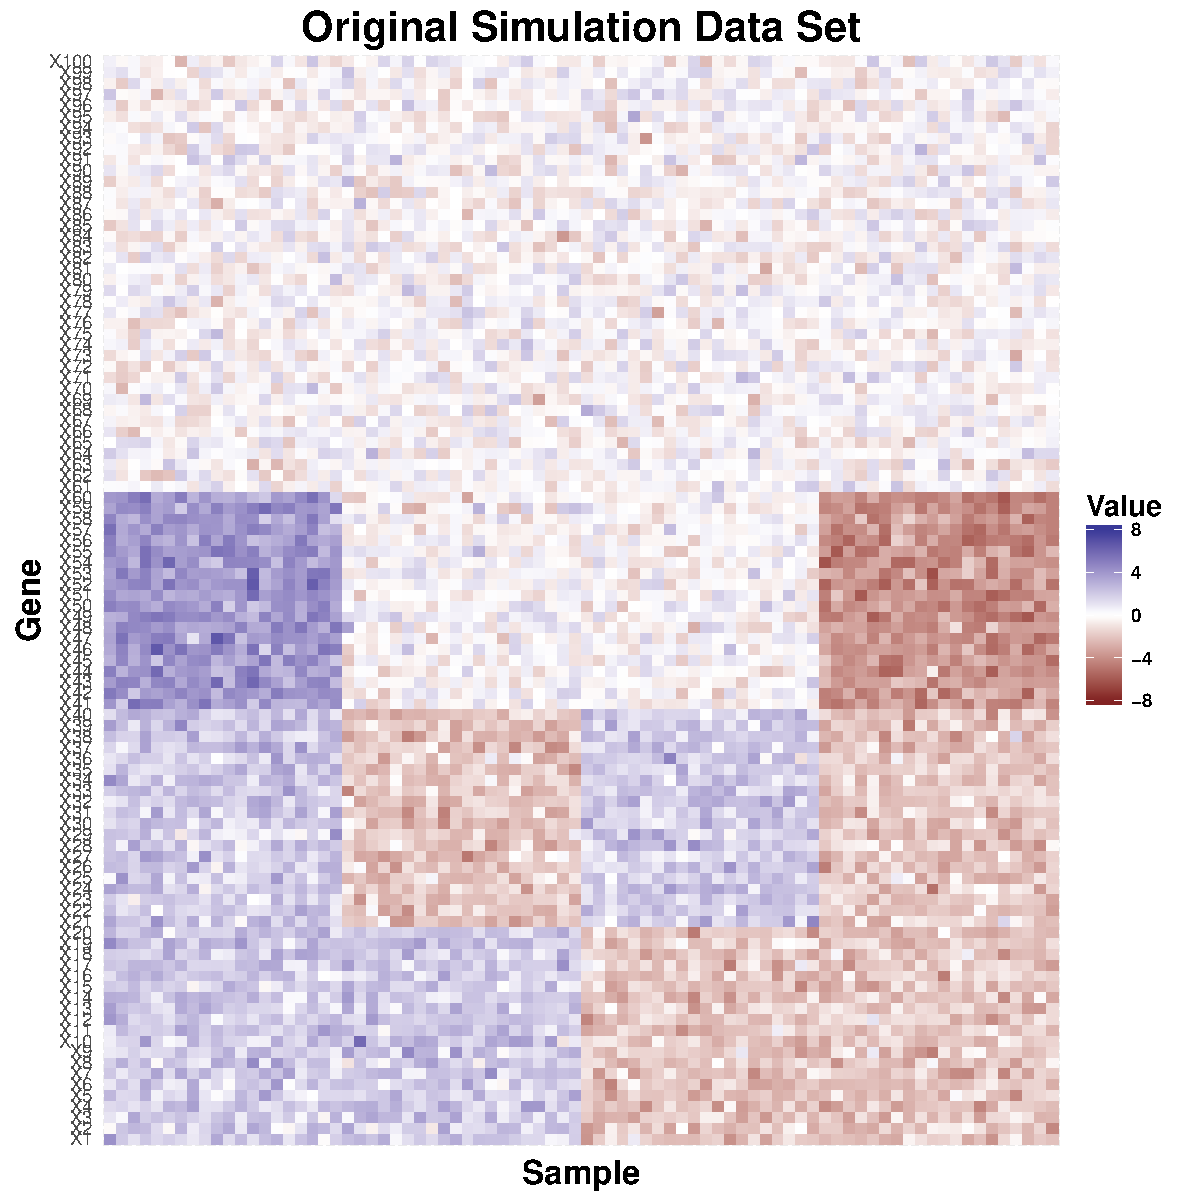
\includegraphics[width = \textwidth]{figures/simulate2.pdf}
        \caption{Original simulation data set in the Case 2}
        \label{fig:data2}
    \end{subfigure}% 
~
    \begin{subfigure}[b]{0.31\textwidth}
        \centering
        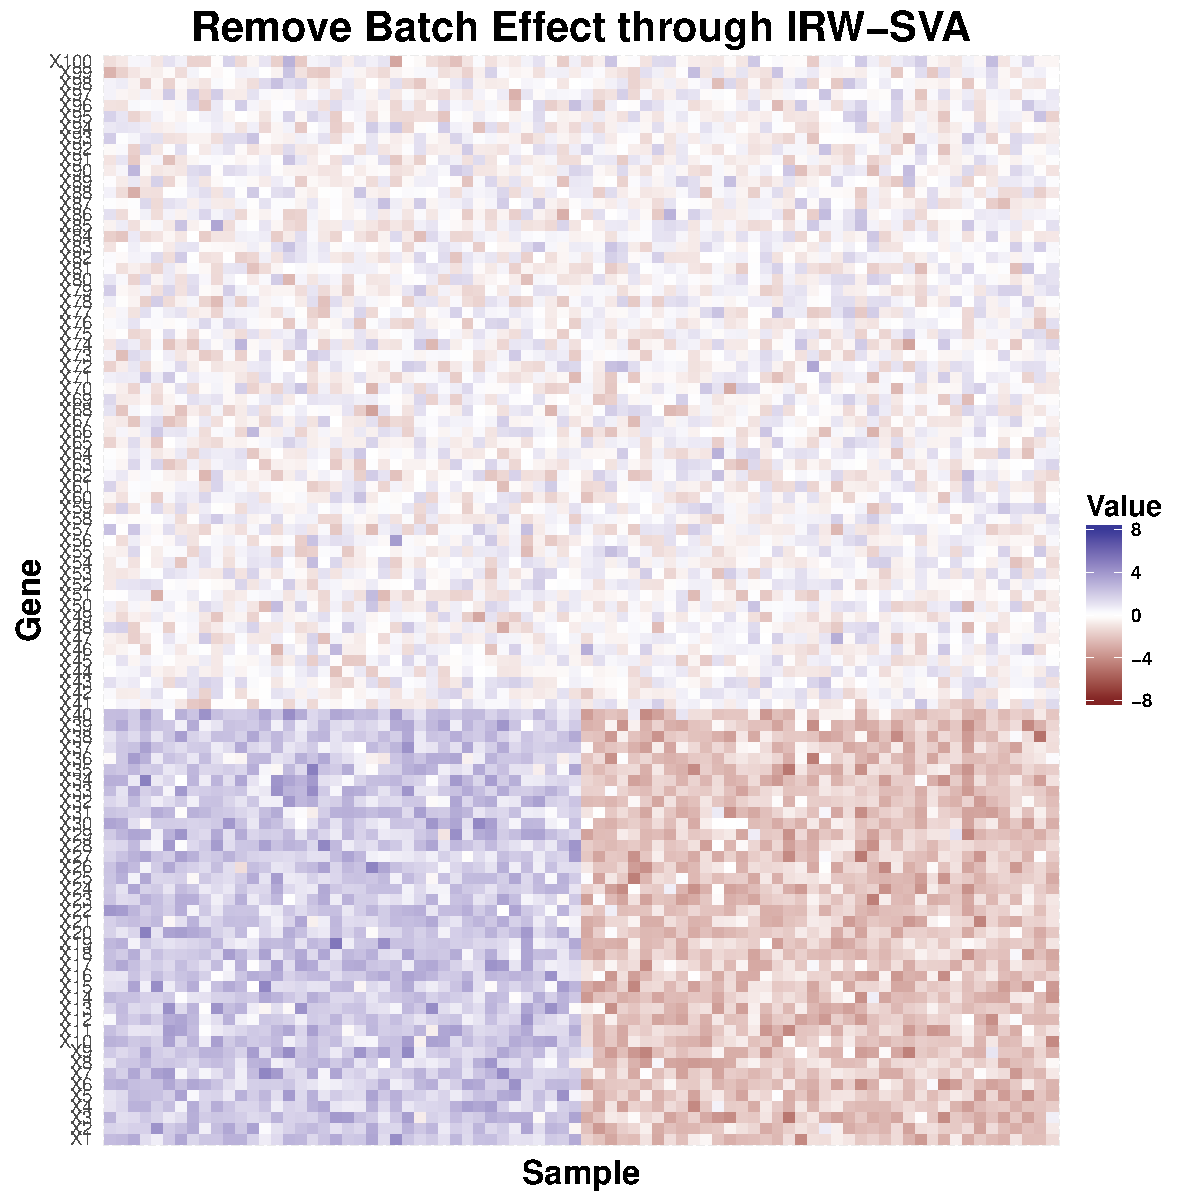
\includegraphics[width = \textwidth]{figures/sva2.pdf}
        \caption{Batch adjustment by IRW-SVA}
        \label{fig:sva2}
    \end{subfigure}  %
~
    \begin{subfigure}[b]{0.31\textwidth}
        \centering
        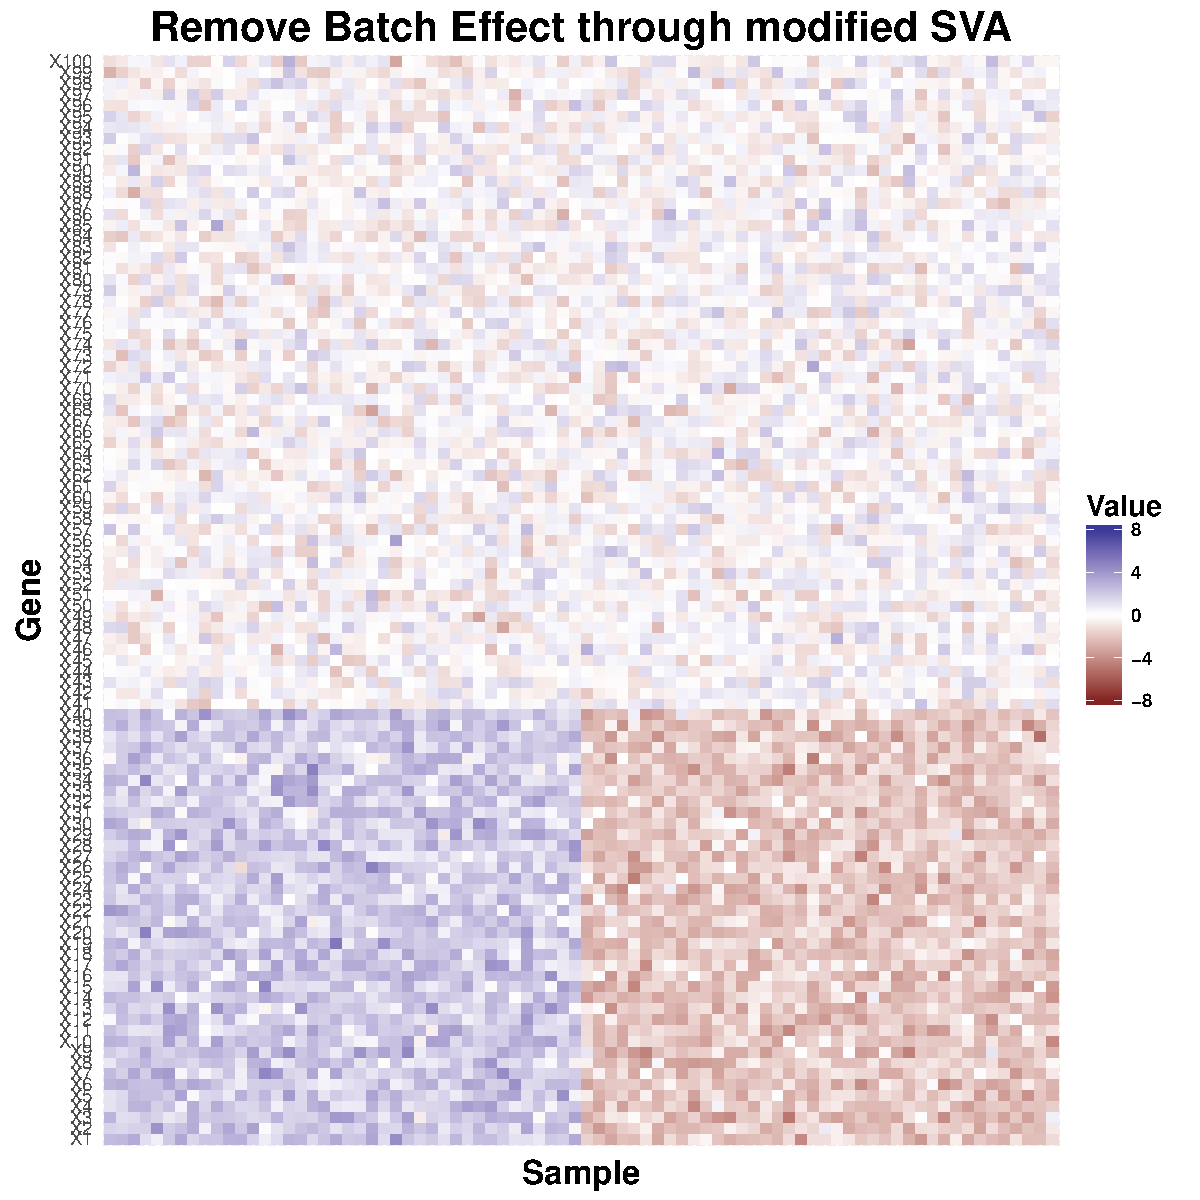
\includegraphics[width = \textwidth]{figures/new_sva2.pdf}
        \caption{Batch adjustment by modified SVA}
        \label{fig:new_sva2}
    \end{subfigure}    
    \caption{Study batch effect through two approaches to SVA in Case 2. Show both approaches to SVA work well in this case.}
    \label{fig:svas2}
\end{figure}




\begin{figure}[h!]
    \centering
    \begin{subfigure}[t]{0.45\textwidth}
    \centering
    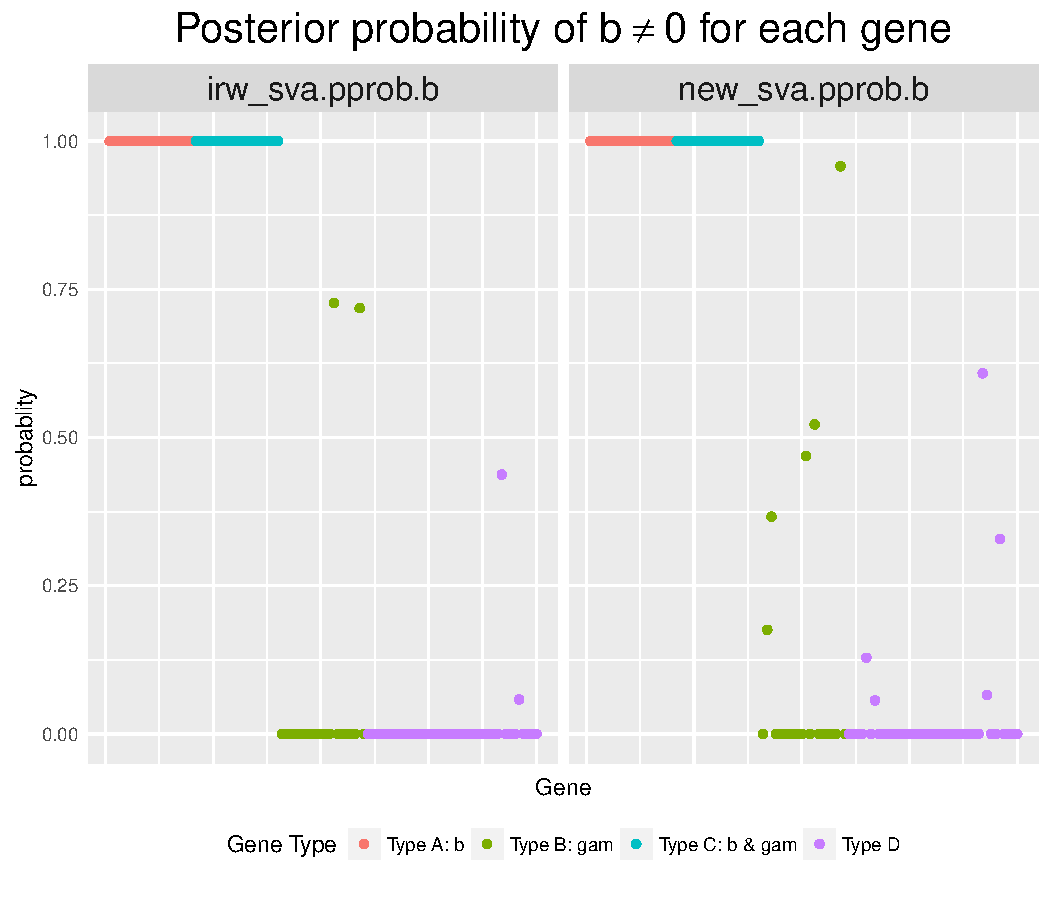
\includegraphics[width = \textwidth]{figures/pprop2_2.pdf}
    \caption{Posterior probability of genes affected by class label (measured factor).}
    \label{fig:pprob2_1}
    \end{subfigure}
    ~
     \begin{subfigure}[t]{0.45\textwidth}
    \centering
    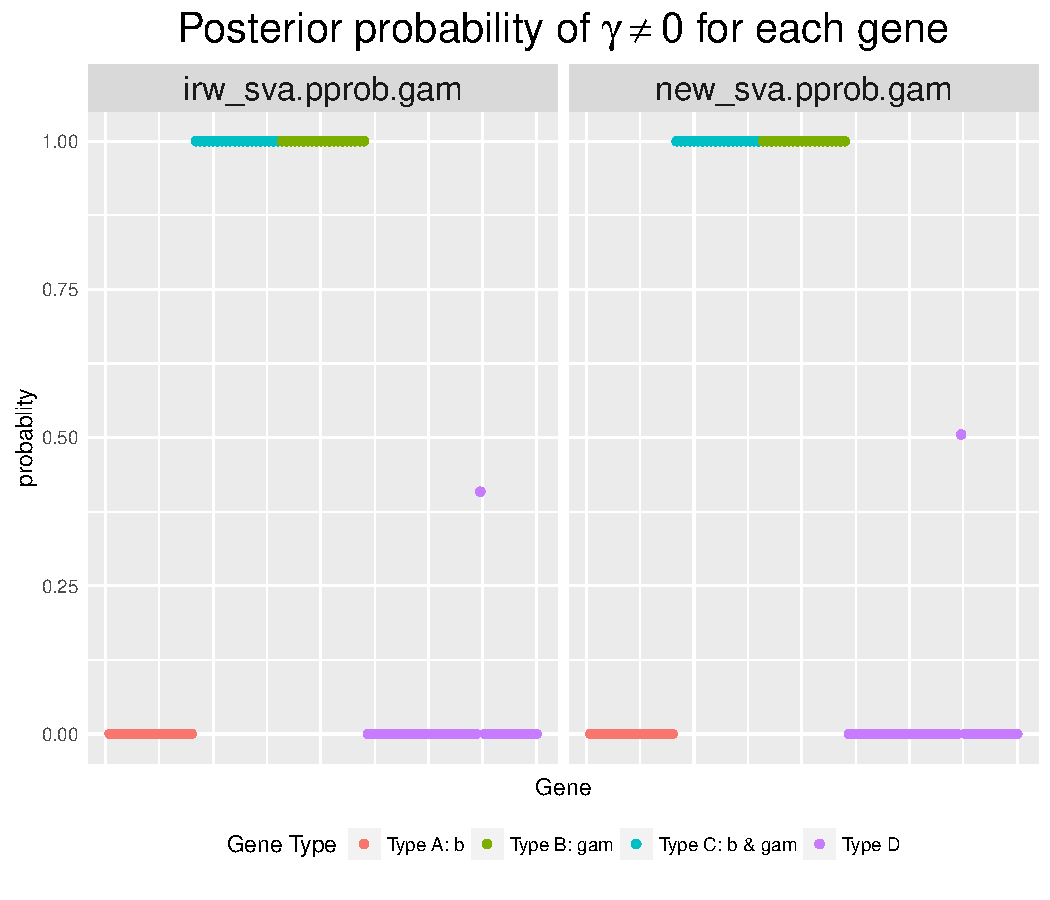
\includegraphics[width = \textwidth]{figures/pprop2_1.pdf}
    \caption{Posterior probability of genes affected by batch label (unmeasured factor).}
    \label{fig:pprob2_2}
    \end{subfigure}
    \caption{The posterior probabilities for genes in the Case 2. In each subfigure, the panels on the left show the results from IRW-SVA and the panels on the right show the results form modified SVA.}
    \label{fig:visual2}
\end{figure}

\begin{figure}
    \centering
    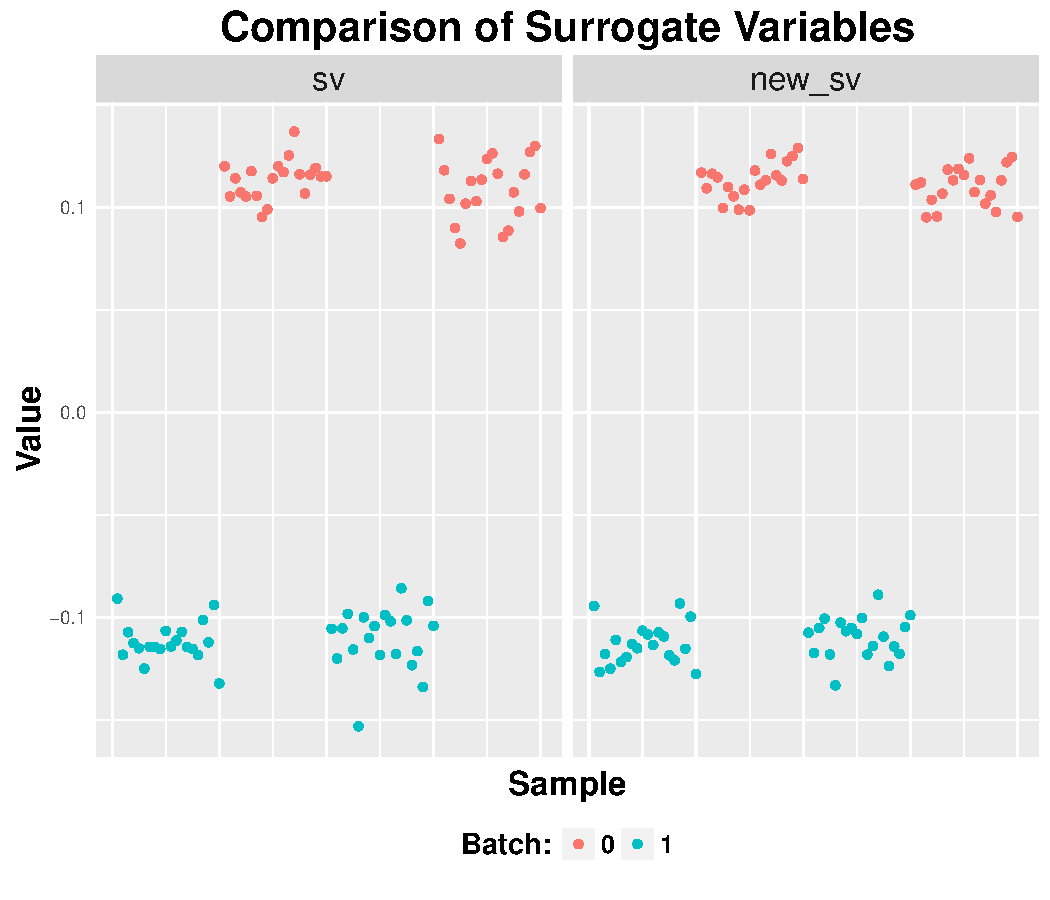
\includegraphics[width = 0.6\textwidth]{figures/vector2.pdf}
    \caption{Comparison of surrogate variables. The left panel shows the surrogate variable constructed through IRW-SVA and the right panel shows the surrogate variable constructed through modified SVA, with both giving good performance.}
    \label{fig:vector2}
\end{figure}

\newpage
\clearpage

\bibliographystyle{plain}
\bibliography{svabib}

\end{document}